\documentclass{beamer}
\usepackage{float}

\usetheme{default}

\title{Text Editors, Vim, and More}

\author{Ethan Oswald Massey\inst{1}}

\institute[]
{
  \inst{1}
  Hochschule Bonn-Rhein-Sieg

}

\begin{document}

\begin{frame}
  \titlepage
\end{frame}

\begin{frame}{Outline}
  \tableofcontents
\end{frame}

\begin{frame}{About Me}
  \section{About Me}

  \begin{itemize}\setlength\itemsep{1em}
    \item Fifth semester HBRS student currently working on my thesis
    \item Graduated from University of Wisconsin-Madison with a double major
      in Computer Engineering \& Computer Sciences
    \item Worked for two years after graduating in the industry doing mostly
      C and C++ work on embedded and systems level projects
    \item Avid Vim user of just under 10 years
  \end{itemize}

\end{frame}


\begin{frame}{Text Editor Overview}
  \section{Text Editor Overview}

  \begin{itemize}\setlength\itemsep{1em}
    \item Text editing vs text viewing
    \item Plugins
    \item Terminal vs GUI
  \end{itemize}

  \begin{itemize}\setlength\itemsep{1em}
    \item GUI
      \begin{itemize}
        \item Atom
        \item Lime (open-source Sublime)
        \item Gedit
        \item Any IDE (VScode, PyCharm, Eclipse, etc)
      \end{itemize}
    \item CLI
      \begin{itemize}
        \item Vim
        \item Emacs
        \item Pico
        \item Nano
      \end{itemize}
  \end{itemize}

\end{frame}


\begin{frame}{Vim}
  \section{Vim}
  \framesubtitle{What is it? Why use it?}

  \begin{itemize}\setlength\itemsep{1em}
    \item A CLI text editor
    \item Unique set of key bindings
    \item Pros
      \begin{itemize}
        \item Efficiency
        \item Power
        \item Ubiquity
      \end{itemize}
    \item Cons
      \begin{itemize}
        \item Steep learning curve
      \end{itemize}
  \end{itemize}

  \framebreak

\end{frame}


\begin{frame}{Vim}
  \framesubtitle{The Basics}

  \begin{itemize}\setlength\itemsep{1em}
    \item Two main modes - Normal (commands) \& Insert (Typing)
    \item Move with \{h, j, k, l\}
    \item Enter insert mode with ``i"
    \item Exit insert mode with [esc]
    \item Undo ``u''
    \item Redo ctrl + ``r''
    \item Save ``:w"
    \item Quit ``:q"
    \item Save \& Quit ":wq"
  \end{itemize}

\end{frame}

\begin{frame}{Vim}
  \framesubtitle{Find \& Replace}

  \begin{itemize}\setlength\itemsep{1em}
    \item Search with ``/" (case sensitive)
    \item Use ``*" or "\#" to search forward/backward current word
    \item ``n" for the next instance
    \item ``N" for the previous instance
    \item Find and replace using sed
    \item e.g. ``:\%s/replace\_me/replaced!/g"
  \end{itemize}

\end{frame}


\begin{frame}{Vim}
  \begin{figure}
    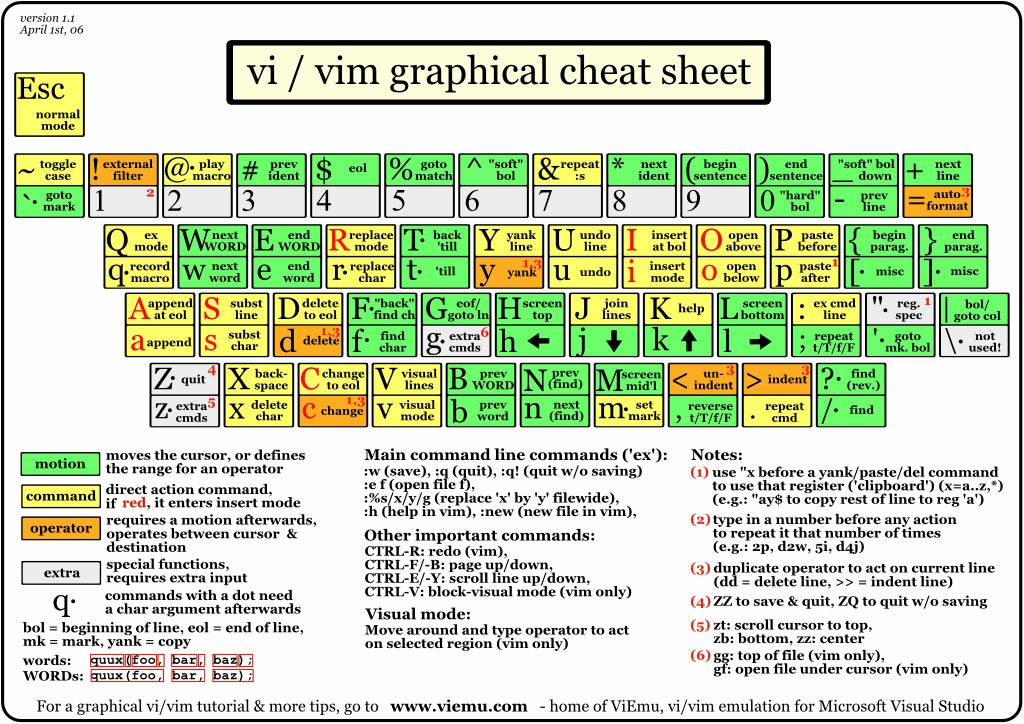
\includegraphics[scale=0.3]{../../resources/vim/vim_cheat_sheet_classic}
    \caption{Classic Vim Cheat Sheet\cite{VimCheatSheet}}
  \end{figure}
\end{frame}



\begin{frame}{Vim}
  \framesubtitle{A Method to the Madness}

  \begin{itemize}\setlength\itemsep{1em}
    \item Vim is a language
    \item Verbs - e.g. {``d''(delete), ``c''(change), ``y''(yank)}
    \item Modifiers - e.g. {NUM, ``i''(inner), ``t''(to), ``f''(from)}
    \item Nouns - e.g. {``w''(word), ``)''(sentence), ``\}''(paragraph)}
    \item The goal is not to memorize random key combinations but to think
      ``I would like to change all the parameters in this function call'' which
      translates to ``ci)``
  \end{itemize}

\end{frame}

\begin{frame}{Vim}
  \framesubtitle{Not convinced?}
  \begin{center}
    {\Huge Demo }
  \end{center}

\end{frame}


\begin{frame}{Vim}
  \framesubtitle{Anti-Patterns \& Things to Avoid}

  \begin{itemize}\setlength\itemsep{1em}
    \item Never use the arrow keys (don't move in insert mode)
    \item Try to avoid using the mouse
    \item Avoid hitting the same key more than a few times (use numbers)
    \item If you are doing an action repeatedly, ask yourself if there's a better way
  \end{itemize}

\end{frame}


\begin{frame}{Vim}
  \framesubtitle{Tips and Goals}

  \begin{itemize}\setlength\itemsep{1em}
    \item ``.'' repeates the last command/action
    \item ``ci'' + {w, (, <, "} is extremly useful
    \item ``gg=G'' will reformat your code
    \item Learn to use visual[Line \& Block] mode
    \item The global buffer can be accessed with ``"+p'' ``"*p''
    \item Alternatively you can paste with ctrl + shift + ``v''

    \item \emph{\textbf{\Large Have patience}}
    \item \emph{\textbf{\Large Learn a new key every few days}}
  \end{itemize}

\end{frame}


\begin{frame}{Closing Thoughts}
  \framesubtitle{General Recommendations for a Development Environment}

  \begin{itemize}\setlength\itemsep{1em}
    \item Take time to customize and explore settings
    \item Play around, break things
    \item Ask others what they use/how they do things
    \item Avoid elitism but don't always do what's easiest
  \end{itemize}

\end{frame}


\begin{frame}{References \& Resources}
  \section{References \& Resources}

  \begin{thebibliography}{10}
    \bibitem{vimCheatSheet}
      \href{https://rumorscity.com/2014/08/16/5-best-vim-cheat-sheet/}{Vim Cheat Sheets}
    \bibitem{What is Vim and Why use Vim?}
      \href{https://medium.com/@fay_jai/what-is-vim-and-why-use-vim-54c67ce3c18e}{What is Vim and Why use Vim?}
    \bibitem{Learning Vim in 2014: Vim as Language}
      \href{https://benmccormick.org/2014/07/02/learning-vim-in-2014-vim-as-language}{Learning Vim in 2014: Vim as Language}
    \bibitem{Learn vim For the Last Time: A Tutorial and Primer}
      \href{https://danielmiessler.com/study/vim/?fb_ref=118ef0e03ab54c0d8197214328648a68-Hackernews}{Learn vim For the Last Time: A Tutorial and Primer}
    \bibitem{Vim anti-patterns}
      \href{https://sanctum.geek.nz/arabesque/vim-anti-patterns/}{Vim anti-patterns}
    \bibitem{Vim Adventures}
      \href{https://vim-adventures.com/}{Vim Adventures}
    \bibitem{Online Vim Tutor}
      \href{https://www.openvim.com/}{Online Vim Tutor}
    \bibitem{Online Vim Tutor}
      \href{https://www.openvim.com/}{Online Vim Tutor}

  \end{thebibliography}

\end{frame}

\end{document}


